\documentclass[letterpaper, 10 pt, conference]{IEEEtran}  % Comment this line out
                                                          % if you need a4paper

% The following packages can be found on http:\\www.ctan.org
\usepackage{tikz}     % For adding axes to plots
\usepackage{graphicx} % For including PDFs
\usetikzlibrary{positioning}
\usepackage{balance} % For balancing the last column.
\usepackage{amsmath} % assumes amsmath package installed
\usepackage{amssymb}  % assumes amsmath package installed

%% Command for creating multiplie-line cells inside a table environment
\newcommand{\multilinecell}[2][c]{%
  \begin{tabular}[#1]{@{}c@{}}#2\end{tabular}}

%% ------------------------------------------
%% Block to make a ``titleheader''
\makeatletter
\newcommand*\titleheader[1]{\gdef\@titleheader{#1}}
\AtBeginDocument{%
  \let\st@red@title\@title%
  \def\@title{%
    \bgroup\normalfont\large\raggedleft\@titleheader\par\egroup
    \vskip1.5em\st@red@title}
}
\makeatother
%% ------------------------------------------

\title{\LARGE \bf Analytic Test Functions for Generalizable
  \\ Evaluation of Convex Optimization Techniques}

\titleheader{IEEE SoutheastCon 2020}

\author{Thomas C. H. Lux$^{1}$, Tyler H. Chang$^{1}$% <-this % stops a space
\thanks{$^{1}$Doctoral candidate, Department of Computer Science, Virginia Polytechnic Institute and State University, Blacksburg, Virginia 24060, USA {\tt\small (tchlux at vt.edu, thchang at vt.edu)}}%
}

\begin{document}

%\documentclass[a4paper, 10pt, conference]{ieeeconf}      % Use this line for a4 paper
\IEEEoverridecommandlockouts                              % This command is only needed 
%% % copyright info
\IEEEpubid{\makebox[\columnwidth]{978-1-7281-6861-6/20/\$31.00~\copyright{}2020 IEEE \hfill} \hspace{\columnsep}\makebox[\columnwidth]{ }}

\maketitle

%%%%%%%%%%%%%%%%%%%%%%%%%%%%%%%%%%%%%%%%%%%%%%%%%%%%%%%%%%%%%%%%%%%%%%%%%%%%%%%%
\begin{abstract}

Convex optimization algorithms such as gradient descent, quasi-Newton
methods, and their variants are designed to find the global minimum of
strongly convex functions. When these algorithms are applied to the
minimization of non-convex functions they offer no robust theoretical
guarantees. Despite the lack of guarantees, many methods still find
good solutions in practice and are widely used in academia and
industry to solve non-convex problems. In this paper, a set of
analytic test functions and transformations are presented that can be
used to quantify the expected performance of optimization algorithms
on difficult (non-convex) optimization problems. The test functions
and transformations in this set are used to compare and evaluate the
convergence rates of stochastic gradient descent, L-BFGS, AdaGrad, and
Adam.

\end{abstract}
%%%%%%%%%%%%%%%%%%%%%%%%%%%%%%%%%%%%%%%%%%%%%%%%%%%%%%%%%%%%%%%%%%%%%%%%%%%%%%%%

\section{Introduction}
\label{sec:introduction}

Convex optimization techniques such as stochastic gradient descent
(SGD), Newton's method, and their variants are widely used in machine
learning applications.  Perhaps most notable is the usage of convex
optimization techniques for minimizing neural network loss functions.
Convex optimization is a well studied field, with many theoretical and
practical guarantees on algorithm convergence when applied to convex
objective functions.  Unfortunately, given the non-convex nature of
most loss landscapes, none of the standard theoretical analyses apply
in the context of neural network training.

Therefore in the context of neural network training, the efficiency of
optimization algorithms is measured empirically.  The common
experiment-based analysis poses an issue for designing effective
optimization algorithms, since often the only way to measure
performance is by running the algorithms on complex real world
problems. Even then, an algorithm that performs well on a handful of
problems is not guaranteed to perform well on other problems.  While
the authors of an optimization algorithm may argue that their
algorithm should heuristically perform better given some class of
neural network loss functions, it is almost impossible to make any
theoretical guarantees.

To address this issue, this work presents a framework for empirical
analysis based on the optimization of four analytic objective
functions. This framework is applied to test four well-known
optimization algorithms.  Each of the four objective functions in this
paper has been carefully designed to exhibit some property that
contrasts with those of a \textit{nice} convex function.  Based on
literature and industry usage, the four optimization algorithms
considered here are SGD \cite{nemirovski2009robust}, L-BFGS
\cite{nocedal1980updating,liu1989limited}, AdaGrad
\cite{duchi2013proximal}, and Adam \cite{kingma2014adam}.  It is our
hope that by empirically analyzing the convergence of optimization
algorithms on hand-crafted analytic objective functions, the effects
of each design decision on convergence can be observed and quantified.
This work offers deeper theoretical insight into how the choice of
optimization algorithm can be effected by the expected properties of
the objective function landscape.

In the following paper, first the four optimization algorithms of
interest are introduced along with a summary of their convergence
properties on convex functions.  Next, four analytic objective
functions are introduced that each have a specific rational and
purpose for testing the expected convergence rate of an optimization
algorithm. Following the objective functions, three meaningful
transformations that can be used to tune the difficulty of an
optimization problem are presented. Next, an experimental methodology
is outlined and applied to the chosen optimization algorithms.
Finally, some experimental results are visualized and interpreted.

\section{Algorithms}
\label{sec:algorithms}

For this analysis, four convex optimization algorithms commonly used
in machine learning are considered, specifically these algorithms are
applied to training neural networks. The four algorithms are SGD,
L-BFGS, AdaGrad, and Adam. A summary of each algorithm along with
theoretical convergence guarantees on convex objective functions
follows.

\subsection{Stochastic Gradient Descent}

SGD \cite{nemirovski2009robust} is a slight modification to the classic
gradient descent algorithm:
$$ x^{(k+1)} = x^{(k)} - \alpha^{(k)} \nabla f\left(x^{(k)}\right) $$
where $x^{(k)}$ denotes the $k$th iterate, $\alpha^{(k)}$ denotes the
$k$th step size, and $\nabla f(x)$ denotes the gradient of $f$ at the
point $x$.  Gradient descent can be thought of as an iterative
minimization of the original function $f$ based on its first-order
Taylor expansion:
$$ f(x) \approx f(x^{(k)}) + \nabla f(x^{(k)})^T x $$
subject to the constraint that $\|x^{(k+1)} - x^{(k)}\| \leq
\alpha^{(k)}/\| f(x^{(k)})\|$.

The difference between SGD and the standard gradient descent
algorithm, is that SGD only assumes access to an approximation $g
\approx \nabla f$.  In theory, the condition on the approximation $g$
is that for all $x$,
$$ \mathbb{E}[g(x)] = \nabla f(x). $$
Because $g$ is an approximation to $\nabla f$, it is possible that
each $g(x^{(k)})$ could actually be an ascent direction, making the
convergence of SGD non-monotone, even for strongly convex functions.
Because of these \textit{bad directions}, for a fixed step size
$\alpha^{(k)} = \alpha$, SGD only converges to within some problem
dependent radius of the true optimum $x^\star$, at which point the
convergence stalls.  To achieve further convergence, the step size
must be decayed.  In practice, $\alpha^{(k)}$ is often held constant
for many iterations, then decayed by some factor $\tau \in (0,1)$.

For a strongly convex function and a deterministic gradient, SGD
reduces to standard gradient descent and its convergence is linear.
I.e., given $t$ iterations,
$$ |f(x^{(k)}) - f(x^\star)| \approx \mathcal{O}\left( c^t ) \right) $$
for some constant $0 < c < 1$.  If $g$ is indeed a stochastic estimate
to $\nabla f$, the convergence rate is reduced to
$\mathcal{O}\left(\frac{1}{t}\right)$.  If furthermore the objective
function is only convex (as opposed to strongly convex), this rate is
further reduced to $\mathcal{O}\left(\frac{1}{\sqrt{t}}\right)$.

\subsection{L-BFGS}

In general, quasi-Newton methods use an approximation to the Hessian
$\nabla^2 f$ to allow for bigger step sizes in directions of low
variance.  For a perfect quadratic, this allows Newton methods to
\textit{jump} straight to the minima; for strongly convex functions,
this accommodates poorly conditioned objective functions by normalizing
the sub-level sets of $f$.  The classic Newton update can be derived
from a second-order Taylor approximation to $f$, and is given by:
$$ x^{(k+1)} = x^{(k)} - \left(\nabla^2 f(x^{(k)})\right)^{-1}\nabla f(x^{(k)}). $$

The original Broyden-Fletcher-Goldfarb-Shanno algorithm (BFGS)
algorithm iteratively refines an approximation to the Hessian matrix
$H^{(k)}$ by applying Rank-1 matrix updates to its current
approximation, each of which satisfies the secant condition:
$$ H^{(k)}\left(x^{(k)}-x^{(k-1)}\right) = \nabla f(x^{(k)}) - \nabla f(x^{(k-1)}).$$
Intuitively, this can be thought of as iteratively refining the
Hessian based on a planar fit to each observed gradient.  The Newton
update is defined in terms of the inverse Hessian, but BFGS avoids
performing a matrix inversion by leveraging the Rank-1
Sherman-Morrison-Woodbury matrix identity:
$$(H + xy^T)^{-1} = H^{-1} - H^{-1}x(I + v^T H^{-1}x)v^T H^{-1}$$
where $xy^T$ is a Rank-1 matrix, and $I$ is the identity.  By
leveraging this formula, BFGS is able to keep the iteration cost
computationally cheap, since the cost of the Rank-1 update is
significantly cheaper than the cost of matrix inversion.

L-BFGS \cite{nocedal1980updating,liu1989limited} is a slight
modification to BFGS, which further reduces iteration and storage
costs for high-dimensional problems.  Instead of keeping track of the
entire Hessian matrix $H$, L-BFGS stores only the previous $m$ update
vectors ($x$ and $y$ in the Woodbury matrix formula), then
reconstructs each $H^{(k)}$ in each iteration.  If $m=1$, then L-BFGS
is reduced to the secant method.  If $m=k_{max}$ (the max-iteration
cost) then L-BFGS is equivalent to BFGS, though the storage and
computational cost may be greater or lesser depending on whether
$k_{max}$ is greater than or less than the dimension.  For a typical
application, $m$ is strictly less than the dimension, making this a
computationally efficient algorithm.  As a useful consequence, the
memory limit ensures that L-BFGS can accomodate non-constant Hessians.

For a strongly convex objective function, L-BFGS converges
superlinearly to the optimum $x^\star$.  That is, L-BFGS is faster
than linear but slower than the quadratic convergence rate
$\mathcal{O}\left( c^{b^t} \right)$ (where both $c$ and $b$ are
positive numbers less than one).  When convexity assumptions are
dropped, L-BFGS has no convergence guarantees.  In fact, in the
presence of local maxima and saddle-points, most quasi-Newton methods
will converge to both \cite{dauphin2014identifying}.

\begin{figure*}
  \centering
  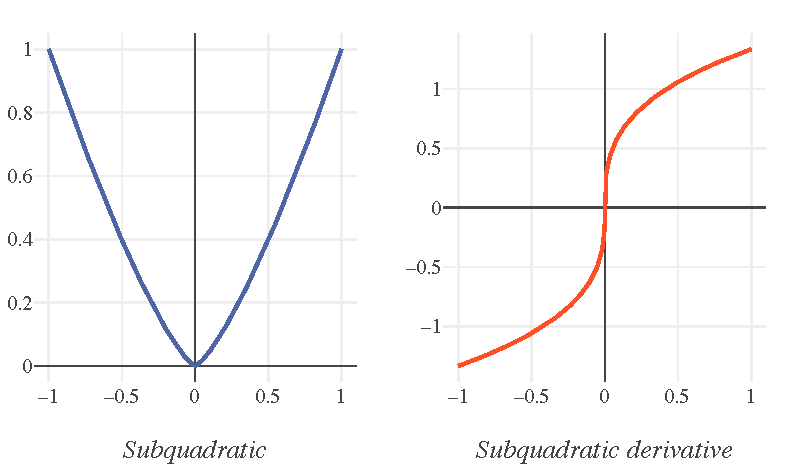
\includegraphics[width=0.45\textwidth]{Figures/final-subquadratic}
  \hspace{5mm}
  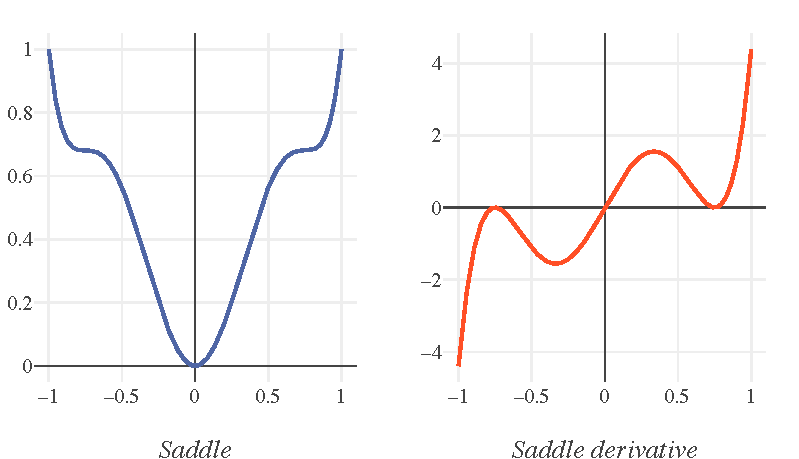
\includegraphics[width=0.45\textwidth]{Figures/final-saddle}
  \\\vspace{5mm}
  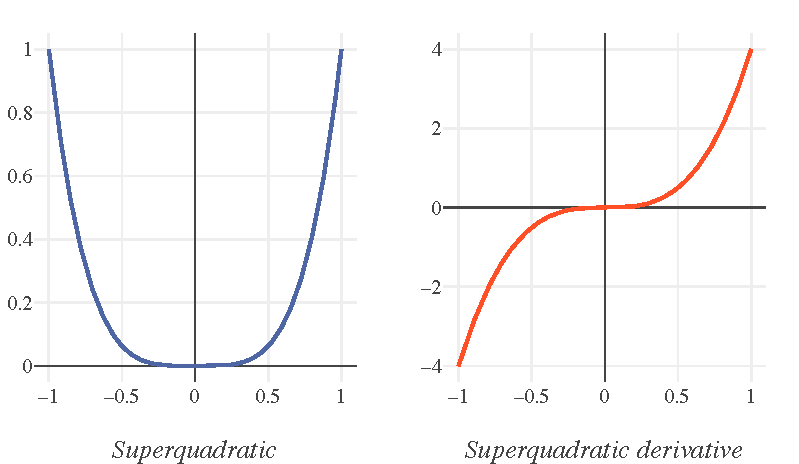
\includegraphics[width=0.45\textwidth]{Figures/final-superquadratic}
  \hspace{5mm}
  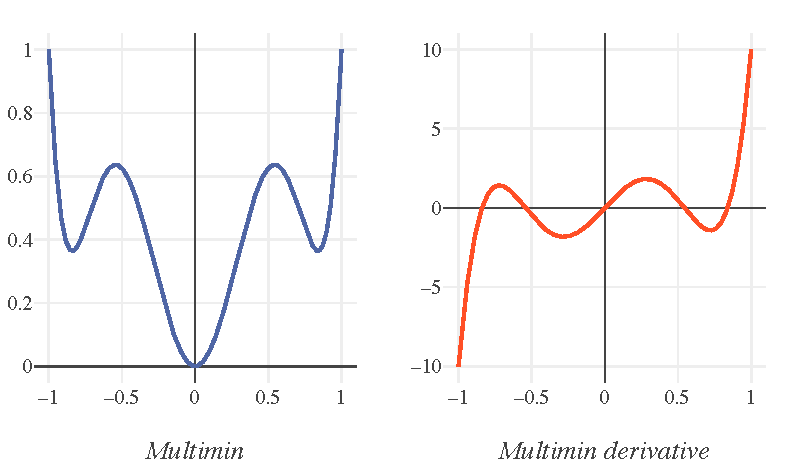
\includegraphics[width=0.45\textwidth]{Figures/final-multimin}
  \caption{One dimensional visualizations of each of the four analytic
    objective functions with derivative adjacent to each
    function. These functions are designed to be extended into many
    dimensions by repeating the same 1D function along each
    component.}
  \label{fig:objectives}
\end{figure*}


\subsection{AdaGrad}

AdaGrad \cite{duchi2013proximal} attempts to recreate the benefits of
Newton's method without explicitly approximating the Hessian.  To
achieve this, AdaGrad directly measures the \textit{variance} in
function value with respect to each basis direction.  Specifically,
AdaGrad derives a variance matrix $G$ that captures the same
approximate information as L-BFGS, but with much lower cost since $G$
is always diagonal given an orthonormal basis.  It should be noted
that for a strongly convex function, the Hessian $\nabla^2 f$ is
always symmetric positive definite (SPD), which immediately implies
that it is columnwise diagonally dominant.  Therefore, for strongly
convex functions, a diagonal matrix $G$ derived from variance
information generally makes a reasonable approximation to the true
Hessian $\nabla^2 f$.

The $k$th variance estimate for each dimension of $G$ is given by
$$ G^{(k)} = diag\left(\sqrt{\sum_{n=1}^k (g^{(n)})^2} + \varepsilon\right) $$

where each $g^{(n)}$ is a previous gradient (estimate) and
$\varepsilon$ is an error-correction factor, introduced to prevent $G$
from becoming singular in degenerate cases.  Note that since $G^{(k)}$
is diagonal, it can be readily inverted.  Also, by storing
$\left(G^{(k)}\right)^2 - \varepsilon I$ and performing the square
root and error-accommodating operations on demand, $G$ can be
iteratively refined without tracking previous gradients.  To normalize
the sublevel sets and improve the conditioning of $f$, a scaled
version of $G$ can be directly plugged in for $H$ in the quasi-Newton
update:
$$ x^{(k+1)} = x^{(k)} - \alpha^{(k)} (G^{(k)})^{-1} g(x^{(k)}) $$
where $\alpha^{(k)}$ is a step size, and $g$ is an approximation to
$\nabla f$ in the stochastic case and $g = \nabla f$ in the
deterministic case.  More intuitively, AdaGrad can also be thought of
as a trust region method, where the variance estimate $G$ allows for
larger steps in directions of low variance.

AdaGrad is guaranteed the same convergence as SGD, but the constant
terms that are ignored by the Big-O notation are siginificantly better
for AdaGrad when the problem is poorly conditioned.

\subsection{Adam}

Adam \cite{kingma2014adam} combines the idea of variance estimation
from AdaGrad, with the idea of momentum.  Intuitively, momentum places
some weight on previous iterates by replacing the current gradient
estimate $g$ with a weighted average of $g$ and the previously seen
gradients:
$$ \hat{g}^{(k+1)}(x^{(k)}) = \beta g(x^{(k)}) + (1-\beta)\hat{g}^{(k)}. $$
When $g$ is a stochastic estimate, this has the effect of smoothing
over noise and avoiding wild oscillations. For poorly conditioned
problems, this prevents the iterates $x^{(k)}$ from wildly oscillating
about the optimum descent direction; for non-convex functions, this
can allow Adam to step through sharp minima, which often correspond to
poor generalization error.

Leveraging the variance estimate $G$ used by AdaGrad, Adam applies
momentum not only to the gradient (first moment) estimate, but also
applies momentum to the variance matrix $G$ (second moment).
Therefore, the Adam update can be summarized by:
\begin{align*}
  x^{(k+1)} &= x^{(k)} - \alpha \left(\sqrt{\beta_2 g^2(x^{(k)}) + (1-\beta_2)(G^{(k)})^2}\right)^{-1}\\
  &\quad\cdot\left(\beta_1 g(x^{(k)}) + (1-\beta_1)\hat{g}\right)
\end{align*}
where $\beta_1$ and $\beta_2$ are the first and second moment
coefficients respectively, and $G^{(k)}$ is the $k$th non-corrected
variance estimate from AdaGrad.  Large momentum coefficients are most
helpful for noisy and poorly conditioned problems.  However, if the
momentum coefficient is too large with respect to the step size
$\alpha$, Adam can fail to converge.  Most interesting problems are
noisy and poorly conditioned, and most algorithms tend to converge
well for any well-conditioned problem.  So, it is common practice to
set $\beta_1 \approx 1$ and $\beta_2 \approx 1$, then choose the
largest convergent step size $\alpha$.

Similarly to AdaGrad, Adam converges at the same rate as SGD but with
more favorable hidden constants when the problem is poorly
conditioned.

\begin{figure*}
  \centering
  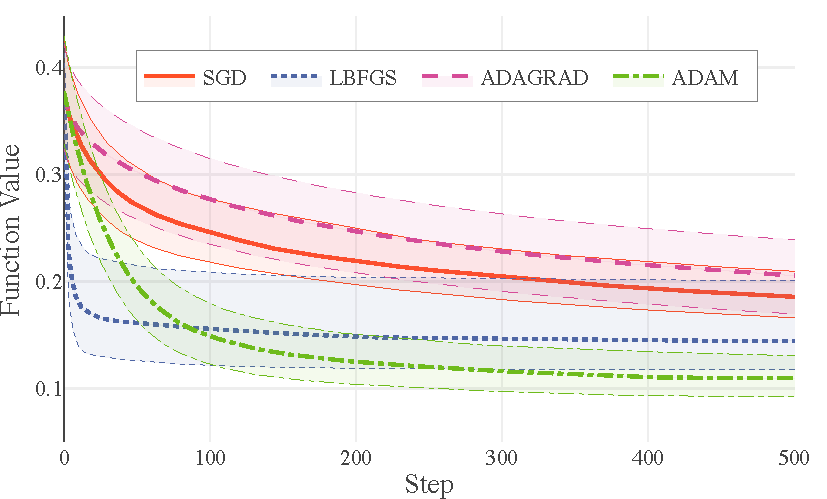
\includegraphics[width=0.45\textwidth]{Figures/final-algorithm-500}
  \hspace{5mm}
  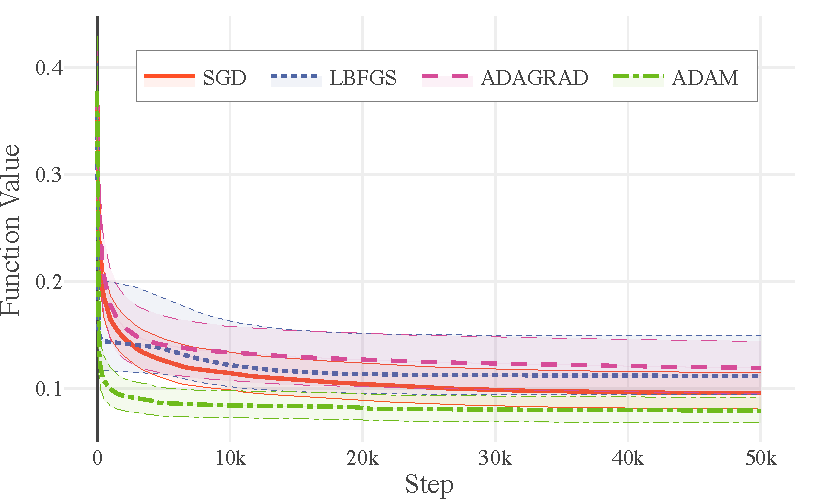
\includegraphics[width=0.45\textwidth]{Figures/final-algorithm-50K}
  \caption{Convergence results averaged over all objective functions,
    dimensions, amounts of noise, rotation, and skew. The thickest
    line in each series represents the median, while the thin lines of
    the same style (and color) represent the 10th and 90th
    percentiles. The left figure depicts only the first 500 steps
    while the right figure depicts all 50 thousand steps. Adam and SGD
    are the best performers beyond two thousand steps. L-BFGS
    performs best in the first 50 steps, then remains second to Adam
    until SGD overtakes it at roughly two thousand steps.}
  \label{fig:results-all}
\end{figure*}

\section{Analytic Objective Functions}

In order to empirically evaluate each optimization technique in a
generalizable way, four analytic functions for minimization are
presented.  Each of these test functions has a single global minimum
and specially designed challenges for typical convex optimization
techniques.

\subsection{Sub-quadratic}

The sub-quadratic is a convex function that appears to come to a
sudden point at the global minimum.  Many common optimization
algorithms will tend to overshoot this minimum due to over stepping.
The function is defined as follows
$$ \sum_{i=1}^{d} |x_i|^{\frac{2k}{2k-1}} $$
where $d$ is the dimension of the problem and $k > 1$.  A
one-dimensional plot of the function and its derivative is shown in
Figure \ref{fig:objectives}.

\subsection{Super-quadratic}

The super-quadratic function is a convex function used to mimic a
phenomenon observed in practice where the region surrounding an
optimal point has a gradient whose magnitude goes to zero at a rapidly
decreasing rate.  Visually, this manifests as a \textit{flattening}
surrounding the global minimum.  The function is defined as follows
$$ \sum_{i=1}^{d} x_i^{2k} $$
where $d$ is the dimension of the problem and $k > 1$.  A
one-dimensional plot of the function and its derivative is shown in
Figure \ref{fig:objectives}.

\subsection{Saddle}

In problems with tens or more dimensions, the likelihood of
non-uniform curvature between dimensions becomes increasingly likely.
When dimensions have opposing curvature, {\it saddle points} are
created.  Recent work \cite{dauphin2014identifying} has shown that
saddle points are a very common occurrence when training neural
networks.  Analytically we define the following function that has
exponentially more saddle points with growing dimension.
$$ \sum_{i=1}^{d} \frac{s^4 x^2}{2} - \frac{s^2 x^4}{2} + \frac{x^6}{6}, $$
where $d$ is the dimension of the problem and $s$ is the constant
defining the absolute value of the location of saddle points
per-dimension.  A one-dimensional plot of the function and its
derivative is shown in Figure \ref{fig:objectives}.

\subsection{Multimin}

Many problems that require optimization have local minima. Using
Chebyshev polynomials, a function is constructed that has a prescribed
number of local minima whose occurrence grows exponentially with
increasing dimension.
$$ \sum_{i=1}^{d} \big [  1 + a x_i^2 + f_{2m + 1}(x_i) \big ], $$
\begin{align*}
  f_0(x_i) &= 1, \\
  f_1(x_i) &= x_i, \\
  f_{n+1}(x_i) &= 2 x_i f_{n}(x_i) - f_{n-1}(x_i), \\
\end{align*}
Here, $d$ is the dimension of the data, $a$ is a multiplier for
determining the relative effect size of the quadratic term, and $m$ is
the number of local minima per dimension. The number of local minima
in the space will grow as $m^d$. When $m$ is odd there will be one
global minimum; this is recommended.  When $m$ is even there will be
$2^d$ global minimizers. A one-dimensional plot of the function and
its derivative is shown in Figure \ref{fig:objectives}.

\begin{figure*}
  \centering
  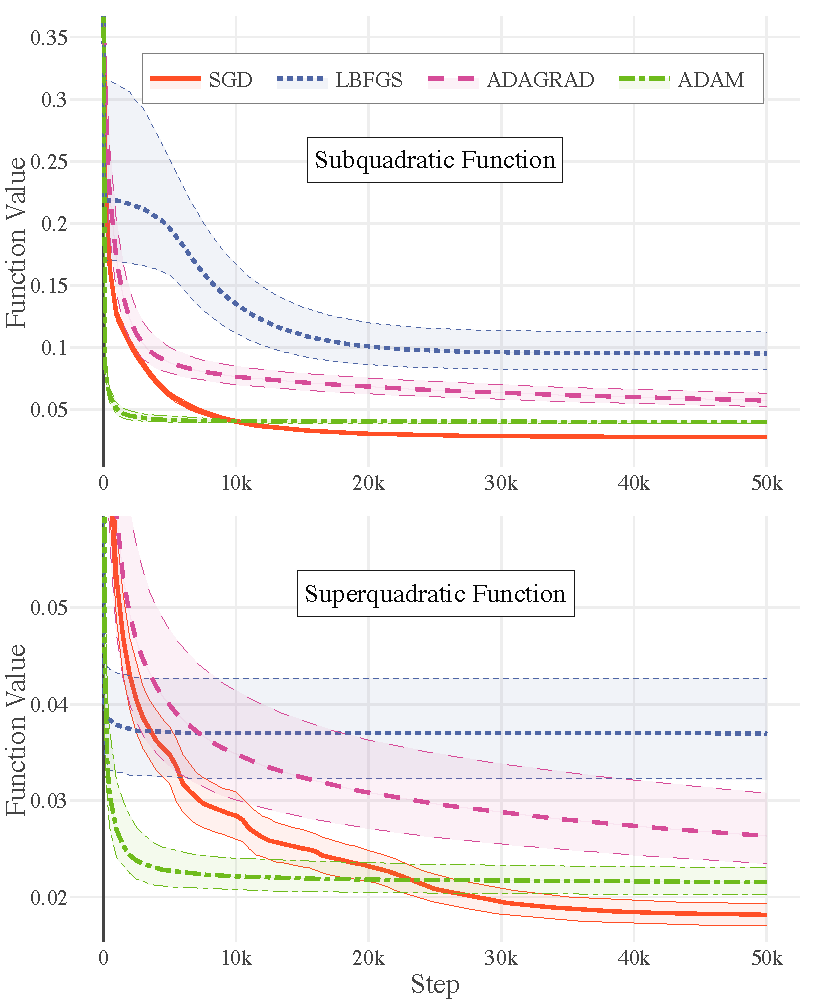
\includegraphics[width=0.45\textwidth]{Figures/final-function-1}
  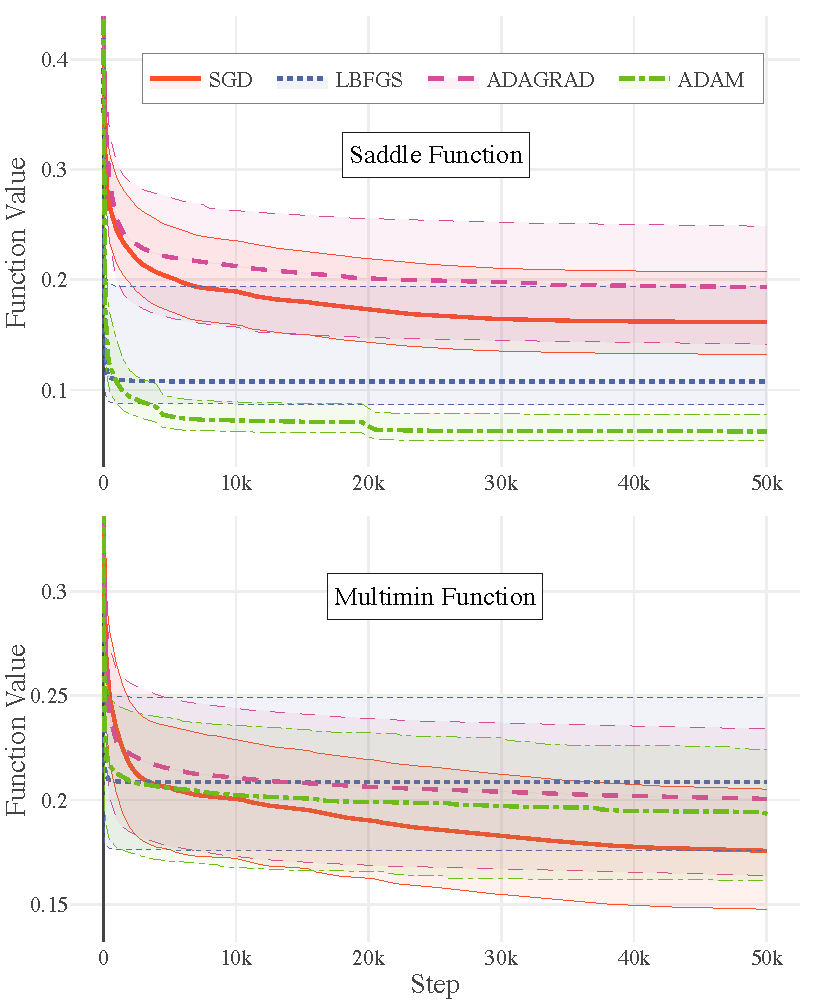
\includegraphics[width=0.45\textwidth]{Figures/final-function-2}
  \caption{Convergence results broken up by function and averaged over
    all dimensions, amounts of noise, rotation, and skew. The thickest
    line in each series represents the median, while the thin lines of
    the same style (and color) represent the 10th and 90th
    percentiles. Adam converges more quickly, but is overtaken by SGD
    after tens of thousands of steps for the sub- and super-quadratic
    functions. Adam and L-BFGS perform best on the saddle objective,
    while SGD and Adam perform best for the multi-minimum objective.}
  \label{fig:results-function}
\end{figure*}

\section{Function Transformations}

Along with the four different objective functions, three analytic
transformations are presented that allow for careful tuning of both
the type and the difficulty of challenges presented to convex
optimization techniques. These three transformations are chosen to
mimic common problems faced in real-world applications.

\subsection{Noise}

The analytic functions that have been presented thus far all have
well-defined, with deterministic gradients almost everywhere.  In most
neural network training applications, a subset of the total training
data volume is used in each gradient evaluation, resulting in a
stochastic estimate of the true gradient.  To simulate this reality,
various amounts of uniform random noise are added to each gradient
evaluation.  SGD and other first order methods (such as Adam and
AdaGrad) are expected to still converge under these conditions
\cite{nemirovski2009robust}.  Though the analysis mentions no
constraint on the variance of the noise, the maximum magnitude of the
uniform noise has been selectively capped at 25\% of the maximum
magnitude of the gradient for our evaluations.  Let $\|g\|_{L^\infty}$
denote the maximum magnitude of the gradient.  For each objective
function, optimizations are attempted with no noise, uniform noise
with 12.5\% of $\|g\|_{L^\infty}$, and uniform noise with 25\% of
$\|g\|_{L^\infty}$. These three amounts of noise are further referred
to as $0$ noise, $.5$ (12.5\%) noise, and $1$ (25\%) noise.

\subsection{Skew}

The condition number of the sub-level set $C$ of a function $f$ is
defined as the ratio between the maximum diameter $W_{max}$ and the
minimum diameter $W_{min}$ across $C$:
$$ \kappa(C) = \frac{W_{max}}{W_{min}}.$$

For $f$ convex, this is proportional to the conditioning of $f$ as an
operator.  Notice that the sublevel sets for all the presented
objective functions are approximately square.  This means that without
modification, the problems are all well-conditioned, i.e., $\kappa(f)
\approx 1$.  To simulate poor problem conditioning, which is common in
machine learning applications, various amounts of skew are introduced
on $f$.  For each objective function, optimizations are attempted with
no skew, an inverse conditioning ratio of $\frac{W_{min}}{W_{max}} =
0.5,$ and an inverse conditioning of $\frac{W_{min}}{W_{max}} = 0.01.$

\subsection{Rotation}

Finally note that each of the presented objective functions is
completely separable, in that it can be decomposed into the sum of its
components in each dimension, which can be optimized separately.  For
Adam and AdaGrad, which use diagonal matrices to capture variance in
each basis dimension, this means that all the necessarry information
can be captured without need for off-diagonal elements.  However, as
the functions are rotated to a maximum angle of $\pi / 8$ radians, the
objective functions become non-separable, making Adam and AdaGrad's
variance approximations poor proxies for the true Hessian.  To
simulate non-separability, optimization algorithms are applied to each
objective function with no rotation, $\pi / 16$ radian rotation ($.5$
rotation), and full $\pi / 8$ degree rotation ($1$ rotation).

\begin{figure}
  \centering
  \begin{tabular}{|c|c|c|c|c|}
    \hline
    & $m$ & $k$ & $a$ & $s$ \\
    \hline
    Sub-quadratic & N/A & 2 & N/A & N/A \\
    Super-quadratic & N/A & 2 & N/A & N/A \\
    Saddle Point & N/A & N/A & N/A & 0.75 \\
    Mult-Min & 3 & N/A & 2 & N/a \\
    \hline
  \end{tabular}
  \caption{The constants that are used within each objective function. $k$ is the power multiplier used for the sub- and super-quadratic functions. $m$ is the number of minima per dimension in the multi-min objective. And $s$ determines the (positive and negative) locations at which the saddle function will have a directional derivative of zero along each dimension.}
  \label{tab:const}
\end{figure}

\begin{figure}
  \centering
  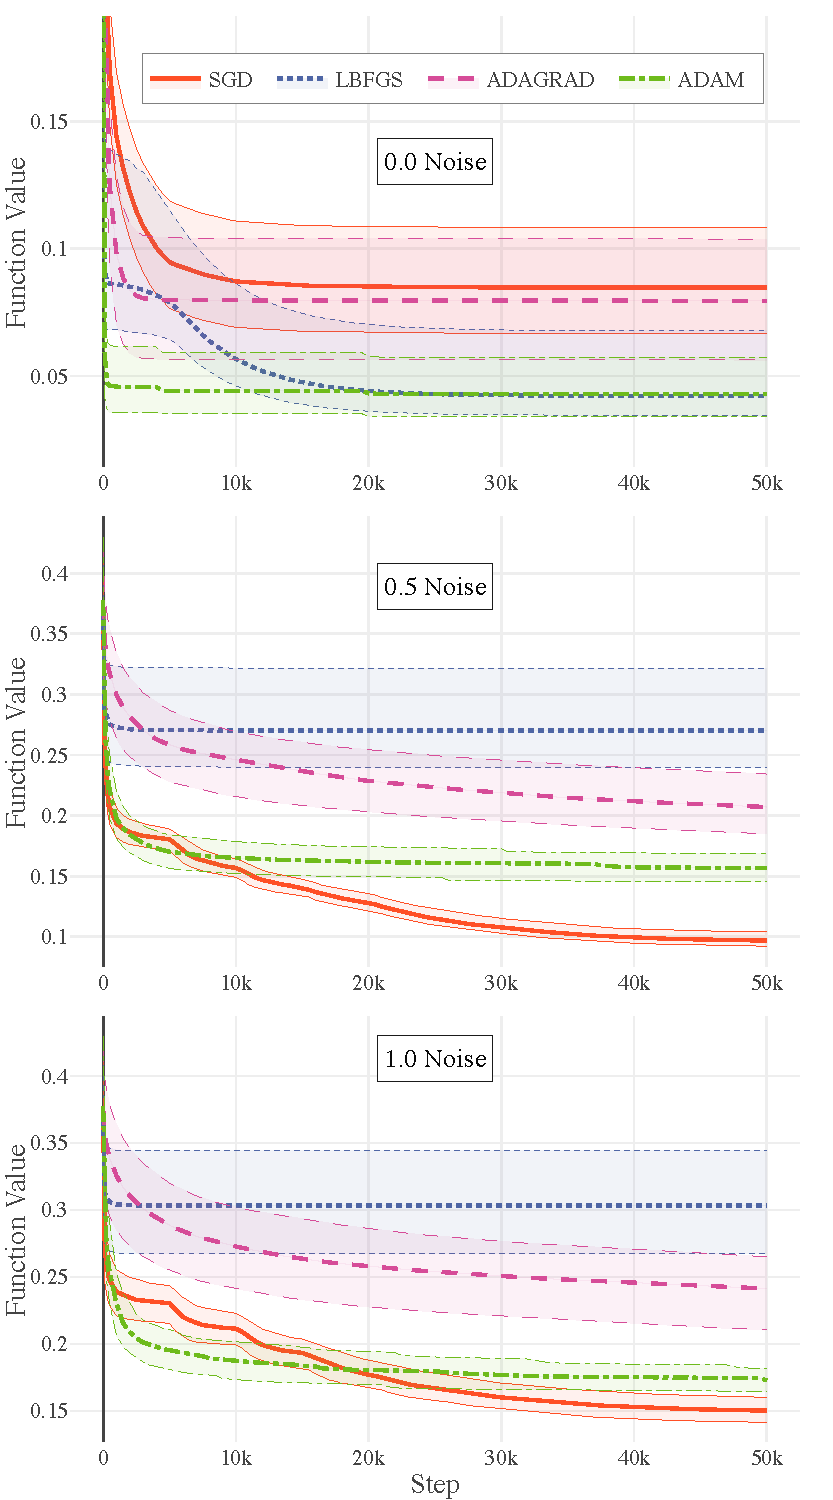
\includegraphics[width=0.5\textwidth]{Figures/final-noise}
  \caption{Convergence results broken up by noise and averaged over
    all functions, dimensions, amounts of rotation, and skew. The
    thickest line in each series represents the median, while the thin
    lines of the same style (and color) represent the 10th and 90th
    percentiles. The introduction of any noise slows the convergence
    of all algorithms while SGD becomes the best. Adam is similar, but
    lacks the later convergence achieved by SGD.}
  \label{fig:results-noise}
\end{figure}

\begin{figure}
  \centering
  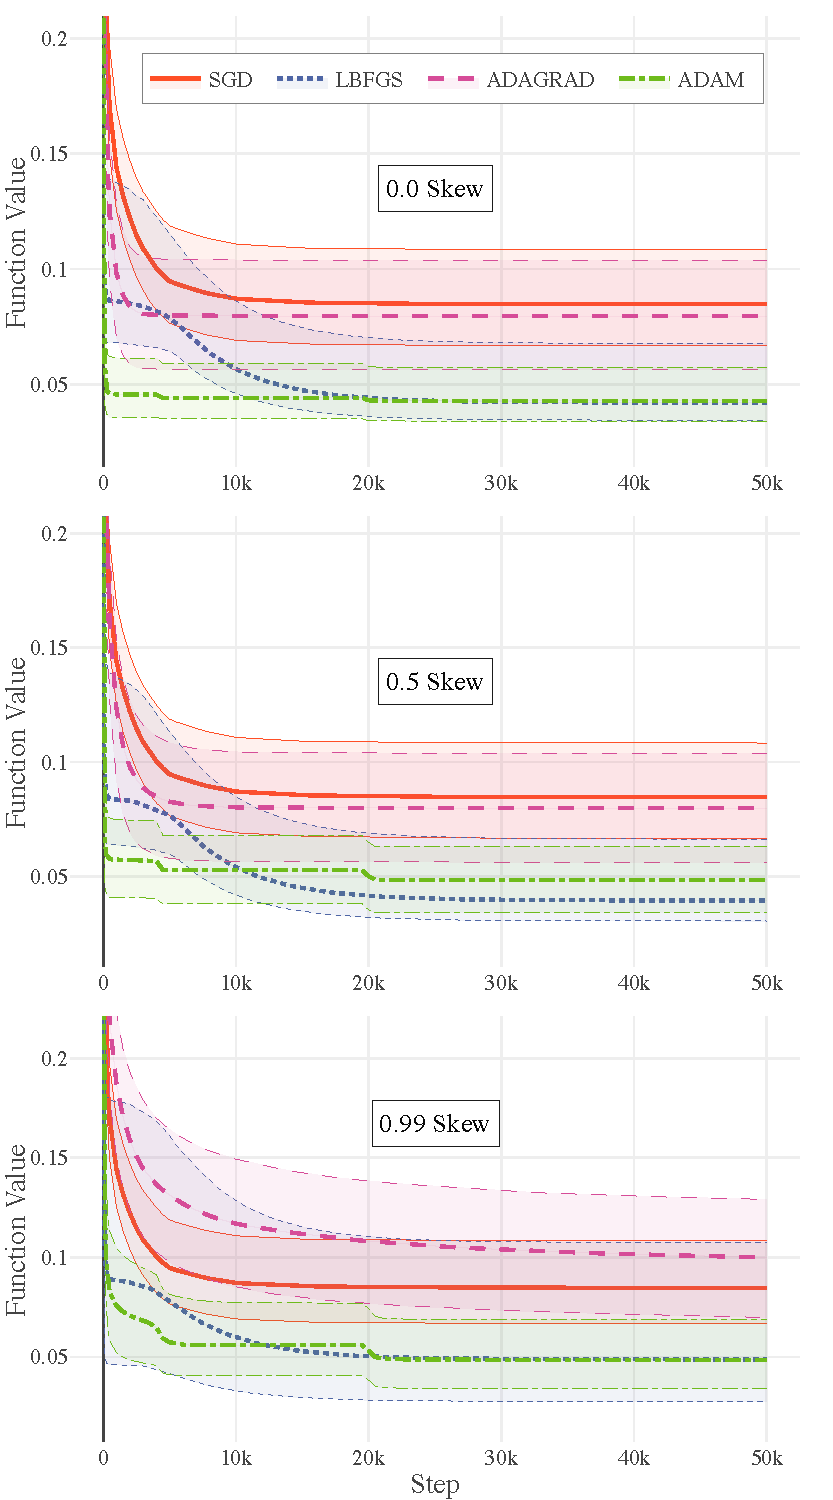
\includegraphics[width=0.5\textwidth]{Figures/final-skew}
  \caption{Convergence results broken up by skew and averaged over all
    functions, dimensions, amounts of noise, and rotation. The
    thickest line in each series represents the median, while the thin
    lines of the same style (and color) represent the 10th and 90th
    percentiles. The existence of mild skew causes L-BFGS to become
    the best technique, while large amounts of skew and no skew both
    lend to Adam remaining the best.}
  \label{fig:results-skew}
  \vspace{1.2cm}
\end{figure}

\begin{figure}
  \centering
  \begin{tabular}{|c|c|c|c|c|c|}
    \hline
    & $\alpha$ & $\beta_1$ & $\beta_2$ & $\tau$ & $\varepsilon$ \\
    \hline
    SGD     & $0.1$  & -- & -- & $0.5$ & -- \\
    L-BFGS & $0.99$ & -- & -- & -- & -- \\
    AdaGrad & $0.01$ & -- & -- & -- & $10^{-6}$ \\
    Adam    & $0.01$ & $0.9$ & $0.99$ & -- & $10^{-8}$ \\
    \hline
  \end{tabular}
  \caption{The hyperparameter settings used for each optimization
    algorithm. The values chosen are those either recommended in the
    source paper, or tuned lightly for this test set (in the case of
    $\alpha$ for SGD). The value of $m$ used for L-BFGS was chosen as
    the maximum of ten and the square root of the dimension.}
  \label{tab:hypeparam}
  \vspace{0.4cm}
\end{figure}

\section{Implementation and Data Collection}

All of the objective functions were implemented in Python, and their
gradients were generated using the Python automatic differentiation
tool {\tt autograd}.  The constants used for the objective functions
are presented in Figure \ref{tab:const}.

The four optimization algorithms discussed have been coded in Python.
For all algorithms the hyperparameter settings were based upon
recommended settings in source papers, specifically for $\beta_1$,
$\beta_2$, $\tau$, and $\varepsilon$, while the step size $\alpha$ was
tuned for reasonable performance. The value of $m$ used for L-BFGS
was chosen as the maximum of ten and the square root of the
dimension. Figure \ref{tab:hypeparam} shows the selected hyperparameter
values for each algorithm.  For SGD, the decay factor $\tau$ was
applied after every five thousand iterations.

Each algorithm was run on each noise level, skew, and rotation
individually for all combinations of all objective functions in
dimensions 10, 100, and 1000. For each objective function and each
level of noise, skew, and rotation, 100 independent trials were run
from (common) random starting points uniformly distributed in the unit
hypercube. The optimization algorithms were permitted 50 thousand
objective function evaluations. Note that each of the four objective
functions has a single global minimum where $f(x) = 0$, and is upper
bounded by $f(x) = 1$.

\section{Results}

The two overall best performers for the analytic objective functions
given varying noise, skew, and rotation were Adam and SGD.  Figure
\ref{fig:results-all} shows the median objective value obtained versus
number of steps for each optimization algorithm over all test
functions and values for noise, skew, and rotation.

The results are broken up by function in Figure
\ref{fig:results-function}, where multiple (expected) behaviors of
each optimization algorithm can be observed. For the sub- and
super-quadratic functions, the decreasing step size of SGD allows
better tail convergence than any other technique. Adam performs best
on the saddle function because its momentum and strictly positive
second-order estimate of objective function curvature allow it to
continue walking closer to the minimum without getting stuck at a
local plateau in the gradient. None of the optimization algorithms are
able to successfully minimize the saddle and multi-min problems, as
these are incredibly difficult in high dimension.

Some unexpected and difficult-to-explain behaviors also occur.  It is
unclear why SGD obtains better tail performance than Adam on the
multi-min problem. Perhaps the step size becomes just the right
size to step out of the local minima.

\begin{figure}
  \centering
  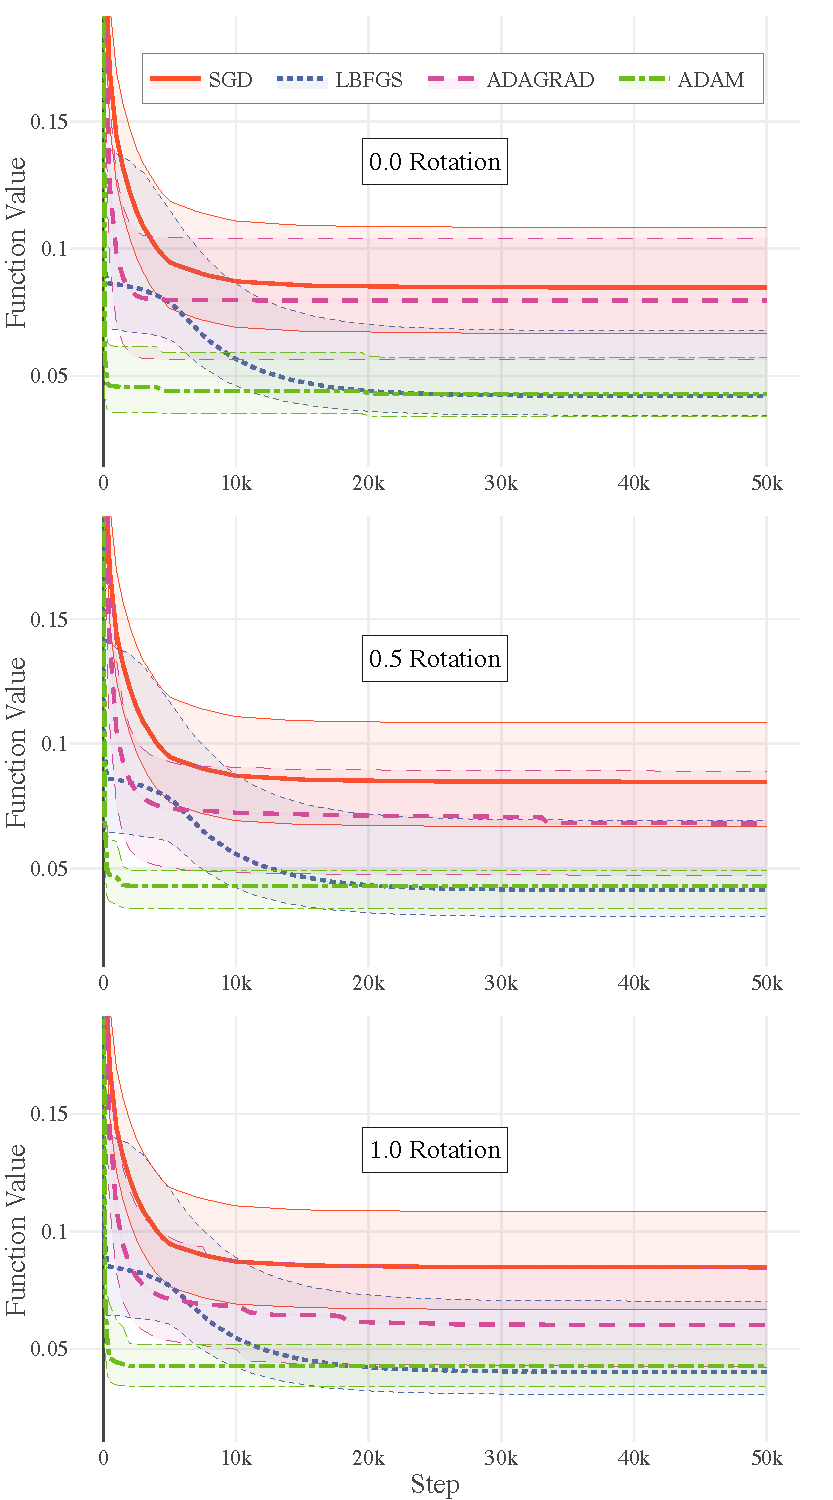
\includegraphics[width=0.5\textwidth]{Figures/final-rotation}
  \caption{Convergence results broken up by rotation and averaged over
    all functions, dimensions, amounts of noise, and skew. The
    thickest line in each series represents the median, while the thin
    lines of the same style (and color) represent the 10th and 90th
    percentiles. The incorporation of rotation has little to no effect
    on the convergence for the evaluated optimization algorithms.}
  \label{fig:results-rotation}
\end{figure}


\subsection{Convergence by Noise}

In Figure \ref{fig:results-noise}, the effect of increased noise in
the gradient of the objective function is studied.

As expected, the addition of noise significantly slows the convergence
of all the algorithms for all the functions.  However, the addition of
noise seems to allow SGD better performance than Adam on average,
especially for amounts of noise that match the hyperparameters of SGD
well (as appears to be the case for a noise of 0.5).

\subsection{Convergence by Skew}

In Figure \ref{fig:results-skew}, the effect of increased skew (i.e.,
deteriorating the conditioning) of the objective functions is studied.

Interestingly, SGD seems to be unaffected by skew. All of Adam,
AdaGrad, and L-BFGS are capable of compensating for skew, so it is
expected that their performance would not be impacted by changing
skew.

\subsection{Convergence by Rotation}

In Figure \ref{fig:results-rotation}, the effect of increased rotation
of the objective functions (which corresponds to non-separability) is
studied.  It was assumed that this could negatively impact Adam and
AdaGrad, but none of the algorithms are significantly affected.

\section{Conclusion}

In this paper, a test set of analytic objective functions and
transformations were presented and used to analyze the convergence of
four common convex optimization algorithms. The specific challenges
posed by the analytic objective functions and the associated
transformations were constructed to match expected behaviors of
real-world problems.  Empirical results confirm common observations
with regards to ADAM and SGD being good choices for non-convex
optimization. However, empirical results also suggest that an initial
burst of 10 to 100 steps of L-BFGS may improve the early convergence
of optimization algorithms in practice. Further theoretical insight
and improved generalizability of results may be allowed by continued
usage of this analytic objective function test set or ones like it.

\balance

\bibliographystyle{IEEEtran}
\bibliography{paper}

\end{document}


